\documentclass[PDF,10pt,usenames,dvipsnames,t,fragile]{beamer}
\usepackage[utf8]{inputenc} % прикручиваем русский язык
\usepackage[russian]{babel}

\usepackage[cm-default]{fontspec} % выбор шрифта (компилить xelatex'ом)
\setmainfont{Century Schoolbook L}
\setsansfont{Arial}
\setmonofont{Consolas}
\everymath{\displaystyle \tt} % математически выражения

\usepackage{hyperref} % поддержка ссылок
\usepackage{tabularx} % нормальные таблицы 

\usepackage{xpatch} % настройка отступов в списках
\xpatchcmd{\itemize}{\def\makelabel}{\setlength{\leftmargin}{3mm}\setlength{\itemsep}{0pt}\def\makelabel}{}{}
\setbeamertemplate{itemize items}[circle] % маркер в списках

\renewcommand{\baselinestretch}{0.9} % межстрочный интервал
\setbeamersize{text margin left=4mm,text margin right=2mm} % отступы
\addtolength{\headsep}{3mm}

\setbeamertemplate{navigation symbols}{} % отключение клавиш навигации

\usepackage{xcolor} % цвета
\usepackage{tikz}
\setbeamercolor{title}{fg=black}
\setbeamercolor{frametitle}{fg=black}

\usepackage{relsize} % вопросительный знак
\newcommand{\bigqm}[1][1]{\text{\rm\larger[#1]{\textbf{?}}}}

\usepackage{ragged2e} % включаем поддержку переносов
%\justifying % включаем переносы

\usepackage{minted} % настройка кода
\usemintedstyle{vs}
\renewcommand{\fcolorbox}[4][]{#4}
\newminted[code]{c_cpp.py:CppLexer -x}{tabsize=4, obeytabs, escapeinside=||}
%\newminted[code]{cpp}{tabsize=4, obeytabs, escapeinside=||}
\newmintinline[lcode]{c_cpp.py:CppLexer -x}{tabsize=4, obeytabs}

\newcommand{\prblm}[1]{{\bigqm[1]} {#1 \\} \vspace{-6pt} \\} % задача (inline)
\newcommand{\inp}{\vspace{4pt}\\ \vspace{4pt}{\bf Входные данные} \\} % заголовок input для задач
\newcommand{\out}{\vspace{4pt}\\ \vspace{4pt}{\bf Результат работы} \\} % заголовок output для задач 
\newcommand{\tb}{\\ \hline} % конец строки в таблице

% таблица с примерами входных данных и результатами работы
\setlength{\extrarowheight}{2pt}
\newenvironment{ex}{\vspace{4pt}\\ \vspace{4pt}{\bf Пример} \\
\tabularx{\textwidth}{|>{\tt}X|>{\tt}X|}
\hline \sf Входные данные & \sf Результат работы \tb}{\endtabularx}

\begin{document}
\begin{frame}[fragile]
	\frametitle{Функции}
	Решение любой задачи естественно стараться свести к решению нескольких
	маленьких подзадач. Если в программе приходится несколько раз выполнять один и
	тот же алгоритм, то имеет смысл выделить его в подпрограмму и вызывать ее при
	необходимости. Такая подпрограмма будет называться {\bf функцией}. \\

	Функция имеет следующий вид:
	\begin{code}
тип имя(список аргументов)
{
	тело функции
}
	\end{code}

	Аргументы перечисляются через запятую с указанием типов. Если аргументов нет,
	ставятся пустые скобки.
\end{frame}

\begin{frame}
	\frametitle{Функции: возвращаемое значение}
	Функции в языке C++ делятся по смыслу на 2 типа.
	\begin{itemize}
		\item Тип \lcode{void}: функция выполняет определённые действия (чтение
			данных, вывод на экран, и т.д.). Точка выхода из функции -- её последняя
			команда или \lcode{return;}
		\item Любой другой тип (\lcode{int, bool, float,} \dots): функция вычисляет
			некоторое значение и {\bf возвращает} его. Точка выхода из функции --
			\lcode{return <значение>;}
	\end{itemize}
	Функции типа \lcode{void} вызываются по её имени со списком аргументов:
	\lcode{	print("hello");}\\
	После имени функции круглые {\bf скобки ставятся обязательно}, даже если
	функция не имеет аргументов. Функция должна быть объявлена до того места, где
	она будет вызвана. \\

	При вызове функций других типов, как правило, сохраняется или используется
	как-то иначе их возвращаемое значение: \\
	\lcode{	int m = max(2, 3);}
\end{frame}

\begin{frame}[fragile]
	\frametitle{Функции: пример}
	\begin{code}
void print(string text)
{
	cout << text << endl;
	// return; — не обязателен
}
int max(int a, int b) // тип нужно указывать у каждого аргумента
{
	// если a > b, функция завершит работу и вернёт значение а
	if (a > b) return a;
	// здесь можно не писать else, т.к. мы попадём сюда только
	// в том случае, если условие не выполнилось
	return b;
}
int main()
{
	print("hello");
	cout << max(4, 2) << endl; // выводим возвращаемое значение
}
	\end{code}
\end{frame}

\begin{frame}
	\frametitle{Количество цифр}
 Дано три символа. Требуется определить, сколько из них являются цифрами. При
	решении данной задачи реализуйте функцию, которая возвращает 1, если символ --
	цифра, и 0 -- иначе.
	\inp
	На вход подаются 3 символа без разделителей.
	\out
	Напечатайте одно натуральное число -- количество цифр.
	\begin{ex}
		123 & 3 \tb
		A5! & 1 \tb
	\end{ex}
\end{frame}

\begin{frame}
	\frametitle{Сумма простых чисел}
	Даны N целых чисел. Определите, какие из чисел являются простыми и
	вычислите их сумму. Также определите, будет ли их сумма простым числом. При
	решении данной задачи реализуйте функцию, которая проверяет одно целое
	число на простоту.
	\inp
	На вход подаётся натуральное число N, далее ещё N целых неотрицательных чисел.
	\out
	На первой строке выведите на экран сумму простых чисел, на второй -- слово <<Yes>>,
	если их сумма -- простое число; иначе слово <<No>>.
	\begin{ex}
		3 \newline 3 5 11 & 19 \newline Yes \tb
		5 \newline 4 2 0 1 9 & 2 \newline Yes \tb
		2 \newline 8 8 & 0 \newline No \tb
	\end{ex}
\end{frame}

\begin{frame}
	\frametitle{Суммы цифр}
	Учительница записала на доске целое число N. Вовочка подсчитал сумму цифр этого
	числа и записал ее ниже. С полученным числом он проделал то же самое, и
	продолжал выписывать числа до тех пор, пока два последних записанных числа не
	совпали. Ваша задача -- найти сумму S всех выписанных на доску чисел. Реализуйте
	подсчёт суммы цифр в числе в виде отдельной функции.
	\inp
	На вход подаётся натуральное число $N \leq 2\cdot 10^9$.
	\out
	Напечатайте натуральное число S.
	\begin{ex}
		34 & 48 \tb
		1234 & 1246 \tb
		987654 & 987711 \tb
	\end{ex}
\end{frame}

\begin{frame}
	\frametitle{Подсчет букв}
 Дано три символа. Требуется определить, сколько из них являются буквами
	латинского алфавита. При решении данной задачи реализуйте функцию, которая
	возвращает 1, если символ -- цифра, и 0 -- иначе.
	\inp
	На вход подаются 3 символа без разделителей.
	\out
	Напечатайте одно натуральное число -- количество букв.
	\begin{ex}
		i23 & 1 \tb
		A5n & 2 \tb
		282 & 0 \tb
	\end{ex}
\end{frame}

\begin{frame}
	\frametitle{В одном шаге от счастья}
 Вова купил билет в трамвае 13-го маршрута и сразу посчитал суммы первых трёх
	цифр и последних трёх цифр номера билета (номер у билета шестизначный).
	Оказалось, что суммы отличаются ровно на единицу. <<Я в одном шаге от
	счастья>>, -- подумал Вова, -- <<или предыдущий или следующий билет точно
	счастливый>>. Прав ли он?
	\inp
	На вход подаётся количество билетов \lcode{N}, далее \lcode{N} шестизначных
	номеров билетов.
	\out
	Для каждого номера выведите на экран \lcode{"Yes"}, если Вова был прав; иначе
	\lcode{"No"}
	\begin{ex}
		3 \newline 715068 \newline 445219 \newline 012200 & Yes \newline No \newline Yes \tb
	\end{ex}
\end{frame}

\begin{frame}
	\frametitle{Секрет}
 Вам в руки попала секретная записка на английском языке. Текст записки может
	быть любым, главное - код, заложенный в тексте. Чтобы расшифровать записку
	нужно посчитать количество букв «b» и «g» в записке (на любом регистре).  Если
	букв «b» больше, чем букв «g», то все плохо. Если букв «b» меньше, чем букв
	«g», то все хорошо. Ну, а если буквы содержатся в записке в одинаковом
	количестве, то пока не ясно, как дела пойдут. Напишите программу для
	расшифровки таких секретных записок.
	\inp
	На вход подаются строки, состоящие из английских букв, цифр, пробелов и знаков
	препинания.
	\out
	Напечатайте все строки в неизменном виде, после на новой строке выведите
	слово, определяющее тайный смысл записки: \\
	<<GOOD>> -- если все хорошо; \\
	<<BAD>> -- если все плохо; \\
	<<NEUTRAL>> -- если пока не ясно, как пойдут дела.
\end{frame}

\begin{frame}
	\frametitle{Секрет}
	\leavevmode
	\begin{ex}
		It is rainy and I have bought umbrella & It is rainy and I have bought
		umbrella \newline BAD \tb
		It is rainy \newline and I have bought tea & It is rainy \newline and I
		have bought tea \newline NEUTRAL \tb
		My aunt Ann is greedy! & My aunt Ann is greedy! \newline GOOD \tb
	\end{ex}
\end{frame}

\begin{frame}[fragile]
	\frametitle{Рекурсия}
	Состояние, в котором функция вызывает сама себя или несколько функций вызывают
	друг друга, называется {\bf рекурсией}. Использование рекурсии часто позволяет
	упростить реализацию алгоритма, однако иногда её использование существенно
	снижает эффективность программы. \\

	Пример рекурсивной функции:
	\begin{code}
unsigned long long fact(int n)
{
	if (n < 2)
		return 1;
	else
		return fact(n-1)*n;
}
	\end{code}
\end{frame}

\begin{frame}[fragile]
	\frametitle{Рекурсия: плохой пример}
	Реализуем рекурсивную функцию, вычисляющую n-ое число Фибоначчи по
	определению: $F_n = F_{n-1} + F_{n-2}$.

	\begin{code}
unsigned long long fib(int n)
{
	if (n < 3)
		return 1;
	else
		return fib(n-1) + fib(n-2);
}
	\end{code}
	Попробуйте вычислить с её помощью 40-ое число Фибоначчи. \\
	В чём причина низкой производительности? \\

	\bigqm \, Перепишите функцию без использования рекурсии.

\end{frame}

\begin{frame}
	\frametitle{Разворот}
	Дано натуральное число N и последовательность из N элементов. Требуется
	вывести эту последовательность в обратном порядке. Для решения задачи напишите
	рекурсивную функцию.
	\inp
	На вход подаётся натуральное число N, за ним ещё N натуральных чисел.
	\out
	Выведите N чисел в обратном порядке.
	\begin{ex}
		3 \newline 1 2 3 & 3 2 1\tb
	\end{ex}
\end{frame}

\begin{frame}
	\frametitle{Рекурсия: задачи}
	При решении следующих задач используйте рекурсию, пользоваться циклами нельзя.
	Все числа в задачах натуральные, их количество не превышает 10000.
	\\

	\prblm{Напечатайте все числа от 1 до n}
	\prblm{Вычислите сумму цифр данного числа}
	\prblm{Выведите цифры числа справа налево через пробел}
	\prblm{Выведите цифры числа слева направо через пробел}
	\prblm{Выведите все нечётные элементы последовательности (0 - признак конца)}
	\prblm{Выведите все элементы последовательности с нечётными номерами (0 -
	признак конца)}
	% https://server.179.ru/tasks/training/recursion.html
\end{frame}

\begin{frame}[fragile]
	\frametitle{Работа с файлами}
	Для работы с файловой системой используется библиотека \lcode{fstream}. Загрузив
	файлы на чтение или на запись с ними можно работать, как с потоками
	(например \lcode{cin, cout}).
\begin{code}
#include <fstream> // библиотека для работы с файлами
#include <iostream>
using namespace std;

int main()
{
	ifstream input("input.txt"); // открыть файл на чтение
	ofstream out("out.txt"); // открыть файл на запись

	if (!input || !out) // ~$x^x$~
	{
		cout << "Ошибка загрузки файла" << endl;
		return 0;
	}

	string s;
	while (getline(input, s))
		out << s << endl;
}
	\end{code}
\end{frame}

\begin{frame}
	\frametitle{Работа с файлами: задачи}
	Создайте файл \lcode{"matrix.txt"} со следующим содержимым:
	{\\ \tt 3 4 \\ 1 2 4 8 \\ 1 3 9 27 \\ 1 5 25 125 \\}
	В первой строке файла заданы размеры матрицы $m \times n$ (количество строк и
	столбцов). Далее идут строки матрицы. \\

	\prblm{Считайте содержимое файла и выведите матрицу на экран}
	\prblm{Запишите матрицу, умноженную на 2, в файл \lcode{"out.txt"}}
	\prblm{Вычислите сумму каждой строки матрицы}
	\prblm{Вычислите сумму каждого столбца матрицы}
\end{frame}

\begin{frame}
	\frametitle{Графы: матрица смежности}
	Рассмотрим следующую матрицу: \\
	{\tt %
	{\color{gray}\nicefrac{i}{j} \hspace{-4pt} 1 2 3 4 5} \\%
	{\color{gray} 1 \,} 0 1 0 0 1 \\%
	{\color{gray} 2 \,} 1 0 0 1 0 \\%
	{\color{gray} 3 \,} 1 0 0 1 1 \\%
	{\color{gray} 4 \,} 0 0 0 0 0 \\%
	{\color{gray} 5 \,} 0 0 1 0 1 \\}

	Единица в позиции $(i,j)$ означает, что между {\bf вершинами} $i$ и $j$
	существует {\bf ребро}. Квадратная матрица, составленная из нулей и единиц,
	называется {\bf матрицей смежности}, которая однозначно задаёт наборы вершин
	$V$ и рёбер между ними $E$: \\
	$V = \{v_1, v_2, v_3, v_4, v_5\}$, \\
	$E = \{(v_1, v_2), (v_1, v_5), (v_2, v_1) \dots, (v_5, v_5)\}$.\\

	Множество, объединяющее эти 2 набора $G = \{V, E\}$, называется {\bf графом}.
	Графы часто используются в программировании: с их помощью удобно задавать
	карты дорог, связи между компьютерами в сети и т.д.

\end{frame}

\begin{frame}
	\frametitle{Матрица смежности: задачи}
	Создайте файл \lcode{"matrix.txt"} со следующим содержимым: \\
	{\tt 5 5 \\ 0 1 0 0 1 \\ 1 0 0 1 0 \\ 1 0 0 1 1 \\ 0 0 0 0 0 \\ 0 0 1 0 1 \\}
	В первой строке файла заданы размеры матрицы $m \times n$ (количество строк и
	столбцов). Далее идут строки матрицы смежности. Будем считать, что матрицей
	задана карта дорог между городами. \\
	\prblm{Подсчитайте общее количество дорог между городами}
	\prblm{Определите, между какими городами есть дороги}
	\prblm{Определите, есть ли прямая дорога из города $i$ в город $j$}
	\prblm{Определите, сколько в графе {\bf концевых вершин}, т.е. городов,
	из которых нет ни одной дороги}
	\prblm{Определите, сколько в графе {\bf изолированных вершин}, т.е. городов
	из которых нет и в которые нет ни одной дороги}
	\prblm{Определите, сколько в графе {\bf петель}, т.е. дорог, ведущих из города
	i в город i}
\end{frame}

\begin{frame}
	\frametitle{Матрица смежности: ещё задачи}
	Создайте файл \lcode{"matrix.txt"} со следующим содержимым: \\
	{\tt 5 5 \\ 0 1 0 0 1 \\ 1 0 0 1 0 \\ 1 0 0 1 1 \\ 0 0 0 0 0 \\ 0 0 1 0 1 \\}
	В первой строке файла заданы размеры матрицы $m \times n$ (количество строк и
	столбцов). Далее идут строки матрицы смежности. Будем считать, что матрицей
	задана карта дорог между городами. \\
	\prblm{Найдите {\bf степени} всех вершин графа, т.е. количество дорог,
	входящих и выходящих из каждого города}
	\prblm{Граф называется {\bf регулярным}, если степени всех его вершин равны.
	Проверьте, является ли заданный граф регулярным}
	\prblm{Граф называется {\bf ориентированным}, если его рёбрам задано
	направление. Проверьте, является ли заданный граф ориентированным}
\end{frame}

\begin{frame}
	\frametitle{Надёжный пароль}
 Будем считать пароль надёжным, если он включает в себя хотя бы одну строчную английскую букву, хотя бы одну заглавную английскую букву и хотя бы одну цифру, при этом его длина должна быть не менее 12 символов. Требуется по данному паролю определить, надёжный ли он. 
	\inp
	На вход программе подаётся одна строка.
	\out
	Выведите на экран "Safe", если пароль надёжный, и "Unsafe" в противном случае.
	\begin{ex}
		VasyaPupkin007 & Safe \tb
		xXx1337xXx & Unsafe \tb
		PupkinVasiliyVasilyevich & Unsafe \tb
	\end{ex}
\end{frame}

\begin{frame}
	\frametitle{IP-адрес}
Для того чтобы выходить в Интернет, каждому компьютеру присваивается так
	называемый IP-адрес. Он состоит из четырех целых чисел в диапазоне от 0 до
	255, разделенных точками. По заданной строке требуется определить, является ли
	она правильным IP-адресом. 
	\inp
	На вход программе подаётся произвольная строка не длиннее 1000 символов. 
	\out
	Выведите на экран "Good", если строка является правильным IP-адресом, и "Bad"
	в противном случае. 
	\begin{ex}
		192.168.1.1 & Good \tb
		1.2.3.4 & Good \tb
		123.456.321.1 & Bad \tb
		1..2.3 & Bad \tb
		1.2.3. & Bad \tb
		10.010.0010.12 & Good \tb
	\end{ex}
\end{frame}

\begin{frame}
	\frametitle{Напёрстки}
 Шулер показывает следующий трюк. Он имеет три одинаковых наперстка. Под первый
	(левый) он кладет маленький шарик. Затем он очень быстро выполняет ряд
	перемещений наперстков, каждое из которых – это одно из трех перемещений - A,
	B, C: \\
	 A - обменять местами левый и центральный наперстки, \\
   B - обменять местами правый и центральный наперстки, \\
   C - обменять местами левый и правый наперстки. \\
Необходимо определить, под каким из наперстков окажется шарик после всех перемещений. 
	\inp
	На вход программе подаётся строка, состоящая из букв A, B, C.
	\out
	Выведите на экран номер напёрстка, под которым окажется шарик: 1, 2 или 3.
	\begin{ex}
		CBABCACCC & 1 \tb
		C & 3 \tb
	\end{ex}
\end{frame}

\begin{frame}
	\frametitle{Цветной дождь}
В Банановой республике очень много холмов, соединенных мостами. На химическом
	заводе произошла авария, в результате чего испарилось экспериментальное
	удобрение. На следующий день выпал цветной дождь, причем он прошел только над
	холмами. В некоторых местах падали красные капли, в некоторых - синие, а в
	остальных - зеленые.  Президенту Банановой республики захотелось покрасить
	мосты между вершинами в цвет холмов, которые они соединяют. Если холмы разного
	цвета, то покрасить мост таким образом не удастся. Посчитайте количество таких
	"плохих"$\,$мостов.  
	\inp  
	В файле {\tt m1.txt} в первой строке записано число холмов $n$, а в следующих
	$n$ строках записана матрица смежности, описывающая наличие мостов между
	холмами. В последней строке записаны $n$ чисел, обозначающие цвета холмов: 1 -
	красный, 2 - синий, 3 - зеленый.
	\out
	Выведите на экран количество "плохих"$\,$мостов.
\end{frame}

\begin{frame}
	\frametitle{Цветной дождь}
	\leavevmode
	\begin{ex}
7 \newline
0 1 0 0 0 1 1 \newline
1 0 1 0 0 0 0 \newline
0 1 0 0 1 1 0 \newline
0 0 0 0 0 0 0 \newline
0 0 1 0 0 1 0 \newline
1 0 1 0 1 0 0 \newline
1 0 0 0 0 0 0 \newline & 4 \tb
	\end{ex}
\end{frame}

\begin{frame}
	\frametitle{Числа-палиндромы}
Палиндромом называется строка, которая одинаково читается как слева направо, так и
справа налево. Рассмотрим все натуральные числа, запись которых в десятичной системе
счисления является палиндромом (при этом запись не начинается с нуля). Например, числа
121 и 1331 являются палиндромами, а число 123 — нет. По данному числу N найдите
N-e в порядке возрастания число-палиндром.
	\inp
	Программа получает на вход одно натуральное число N, не превосходящее 100000.
	\out
Программа должна вывести одно натуральное число --- N-е в порядке возрастания
	число-палиндром.
	\begin{ex}
		20 & 111\tb
	\end{ex}
\end{frame}

\begin{frame}
	\frametitle{Библиотека glcanvas: создание окна}
	Начало координат в окне -- левый верхний угол; ось $X$ направлена влево, ось
	$Y$ -- вниз. Функция принимает размеры окна в пикселях; размер по умолчанию:
	$640 \times 480$ пикселей. \\
	\lcode{void window(int w = 640, int h = 480)}

\tikz [remember picture,overlay]
    \node at ([yshift=-40pt,xshift=0pt] current page.center) 
			        {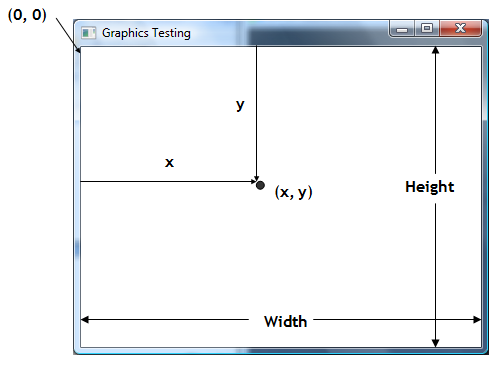
\includegraphics[scale=0.5]{window.png}};
\end{frame}

\begin{frame}[fragile]
	\frametitle{Функция прорисовки}
	Все операции, связанные с прорисовкой графики, нужно помещать внутри одной
	функции. В \lcode{main} эту функцию необходимо специально
	"зарегистрировать"$\,$ как \lcode{glutDisplayFunc}. После этого функция будет
	вызываться автоматически, когда необходимо перерисовать содержимое окна.  Для
	работы с функциями \lcode{glcanvas} нужно подключить саму библиотеку, также
	удобно использовать пространство имён \lcode{cnv}.
	\begin{code}
// минимальный пример
#include <glcanvas.hpp>
using namespace cnv;

void draw()
{
	glutSwapBuffers();
}

int main()
{
	window();
	glutDisplayFunc(draw);
	glutMainLoop();
}
	\end{code}
\end{frame}

\begin{frame}[fragile]
	\frametitle{Основные функции}
	\begin{code}
void draw()
{
	// очистка экрана (цвет фона)
	clear(255, 255, 255);
	// окружность и круг (координаты центра и радиус)
	circle(100, 100, 20);
	circle_fill(240, 175, 25);
	// прямоугольники (координаты двух углов)
	rect(120, 150, 200, 450);
	rect_fill(500, 300, 520, 320);
	// отрезки (координаты концов)
	line(40, 40, 80, 80);
	line(80, 80, 20, 80);
	line(20, 80, 40, 40);
	// вывод текста
	position(300, 300);
	text_out << "Hello, world!";
	// вывод содержимого буфера в окно
	glutSwapBuffers();
}
	\end{code}
\end{frame}

\begin{frame}
	\frametitle{Цвет}
	Цвет в формате RGB задаётся тремя компонентами (красный, зелёный, синий). Он
	может быть записан двумя способами: как тройка десятичных чисел
	\lcode{(r,g,b)} от 0 до 255 или как одно шестнадцатеричное число $0xrrggbb$, в
	котором каждый байт содержит соответствующую компоненту. \\
	\tikz [remember picture,overlay]
			\node at ([yshift=20pt,xshift=0pt] current page.center) 
								{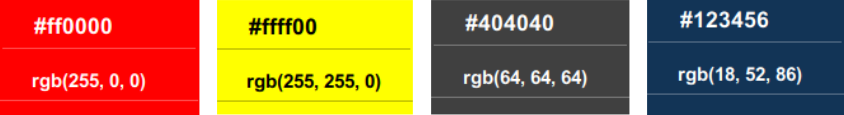
\includegraphics[scale=0.5]{hex.png}};
	\vspace{50pt} \\
	В glcanvas цвет по умолчанию -- чёрный. Изменить его можно функциями
	\lcode{color(hex)} и \lcode{color4(r, g, b)}. Кроме того, в функции рисования фигур
	(circle, rect и т.д.) можно передать цвет в формате HEX последним
	аргументом:\\
	\lcode{circle(100, 200, 40, 0xff0000);} \\
	Для перевода цвета из RGB в HEX есть функция $hexcolor(r, g, b)$:\\
	\lcode{circle(100, 200, 40, hexcolor(255, 0, 0));}
\end{frame}

\begin{frame}[fragile]
	\frametitle{Мышь и клавиатура, анимация}
	Анимация графики осуществляется путём её перерисовки после некоторого события:
	например, движение мышки, нажатие клавиши на клавиатуре или срабатывание
	таймера. 
	\begin{small}
	\begin{code}
// Реагирует на движение мыши с нажатой кнопкой (перетаскивание)
void glutMotionFunc(void (*func)(int x, int y));
// Реагирует на любое движение мыши
void glutPassiveMotionFunc(void (*func)(int x, int y));
// Реагирует на клики
// button: GLUT_LEFT_BUTTON, GLUT_MIDDLE_BUTTON, GLUT_RIGHT_BUTTON
// state:  GLUT_UP, GLUT_DOWN
void glutMouseFunc(void (*func)(int button, int state, int x, int y));
// Реагирует на нажатие клавиши
void glutKeyboardFunc(void (*func)(unsigned char key, int x, int y));
// В функциях выше x, y - координаты курсора
// Срабатывает по таймеру каждые msecs миллисекунд
void glutTimerFunc(unsigned int msecs, void (*func)(int value), value);
	\end{code}
	\end{small}
\end{frame}

\end{document}
